% ! TeX root = ../../thesis.tex
\chapter{Implementazione}
\label{chapter:implementation}
In questo capitolo vengono affrontati gli aspetti implementativi del sistema, descrivendo le tecnologie e i paradigmi utilizzati.

\vspace*{0.5cm}

La tecnica impiegata nel sistema appartiene alla famiglia di tecniche \textit{structure-based} e si compone macroscopicamente di tre fasi, schematizzate in \Cref{img:03-system-overview}:
\begin{enumerate}
	\item \textbf{Analisi}: i sorgenti sono \textit{parsati}, preprocessati e \textit{tokenizzati};
	\item Una fase opzionale di \textbf{filtraggio};
	\item \textbf{Rilevamento} delle somiglianze.
\end{enumerate}

\begin{figure}[h!]
    \centering
    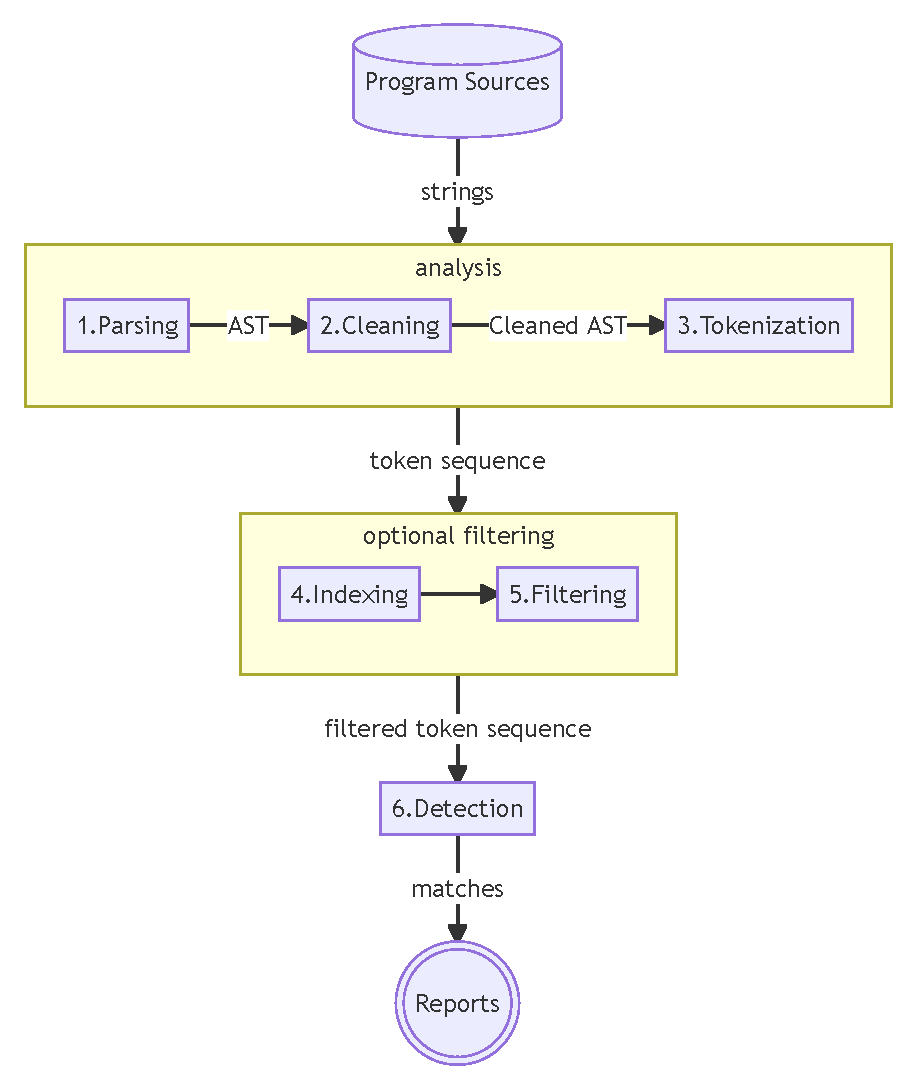
\includegraphics[width=0.8\textwidth]{resources/img/03-system-overview.pdf}
    \caption{Visione d'insieme delle fasi della tecnica impiegata nel sistema in uso.}
    \label{img:03-system-overview}
\end{figure}

Di seguito ciascuna delle tre viene approfondita.

\section{Tecnica di analisi}
Il primo passo consiste nell'effettuare il \textit{parsing} dei sorgenti, affidato alla libreria JavaParser\footnote{\url{https://javaparser.org/}}.
%
JavaParser è una libreria \textit{open source} che permette di effettuare il \textit{parsing} di codice sorgente scritto in linguaggio Java, fornendo comodi meccanismi per l'analisi e la manipolazione dello stesso.

Il risultato del \textit{parsing} è un albero sintattico equivalente a quello mostrato in \Cref{img:01-ast} che rappresenta la struttura dei sorgenti.

Tuttavia, nonostante la generazione dell'albero sintattico sollevi dalla responsabilità di eliminare dal sorgente \textit{token} superflui, come gli spazi e i punti e virgola, in quanto naturalmente modellati dalla struttura stessa dell'albero, tale AST contiene ancora informazioni superflue al fine di identificare codice simile, come le dichiarazioni di \texttt{import} e dei \texttt{package}.
%
Per questo motivo è necessario una fase intermedia di \textit{preprocessing} in cui l'albero viene “sfoltito”. In particolare, in questa fase l'albero viene visitato e, oltre a rimuove le dichiarazioni suddette, sono rimosse anche le funzioni \texttt{hashCode()}, \texttt{equals()} e \texttt{toString()}.
%
Queste, infatti, nella maggioranza dei casi, vengono automaticamente generati dall'\textit{IDE} e non sono rappresentativi della logica dei sorgenti.

A seguire avviene la conversione del codice sorgente in una sequenza di \textit{token}.
%
Si noti che la fase di \textit{tokenizzazione} vera e propria descritta nella \Cref{01-tokenization} è già stata eseguita internamente dal \textit{parser} di JavaParser i cui \textit{token} sono quelli presenti nell'albero.
%
Tali \textit{token}, tuttavia, rappresentano in modo molto specifico la struttura del programma: ...
%
Come descritto nella \Cref{01-tokenization} l'obiettivo è creare invece un insieme di \textit{token} "lasco" che raggruppi tipi di \textit{token} equivalenti a livello semantico.

A questo scopo, l'albero sintattico preprocessato viene visitato e, per ogni nodo, si emette un \textit{token}, con le relative informazioni circa la sua posizione nel sorgente, o meno a seconda sia una dichiarazione semanticamente rilevante o meno.

In particolare, è stato costruito un file di configurazione \textit{Yaml}\footnotetext{Linguaggio, \textit{superset} di Json, per la serializzazione di dati che viene impiegato per la scrittura di file di configurazione: \url{https://yaml.org/}.} (\Cref{lst:token-config-file}) in cui sono elencati i tipi di dichiarazioni rilevanti, eventualmente aggregando tra loro dichiarazione semanticamente simili e che potrebbero essere facilmente cambiate per offuscare la copiatura.
%
Ad esempio, sono state aggregate sotto un unico tipo \texttt{loop-stmt} tutti i costrutti che effettuano un ciclo.
%
In questo modo un cambio sintattico di tipo non sarà sufficiente ad aggirare il sistema perché verrà generato lo stesso tipo di \textit{token}.
%
Si noti che questo approccio è molto flessibile e può essere "aggiustato" a piacimento nel caso sia necessario effettuare una \textit{tokenizzazione} con un insieme di \textit{token} più stringente.

\lstinputlisting[
 	language=yaml,
 	caption={Porzione del file di configurazione con la definizione dei tipi di \textit{token}},
 	label={lst:token-config-file},
]{resources/code/03-token-types.yml}

Il risultato dell'applicazione del processo sopra descritto al \Cref{lst:test-analysis} viene presentato nel \Cref{lst:result-tokenization}

\lstinputlisting[
 	caption={Risultato dell'analisi del \Cref{lst:test-analysis}},
 	label={lst:result-tokenization},
]{resources/code/03-AnalyzedTestAnalysis}

\section{Filtraggio}

\section{Rilevamento delle somiglianze}
Gli algoritmi impiegati per confrontare due sequenze di \textit{token} sono il \textit{Greedy String Tiling} e \textit{Running Karp-Rabin Matching}, che ne rappresenta una sua evoluzione, introdotti da M. Wise nel 1993 in \cite{wise-running-93}.
%
Sebbene questi algoritmi siano stati concepiti per lavorare su sequenze di stringhe, possono essere facilmente riadattati per operare su sequenze di \textit{token}.

Dette $A$ e $B$ due sequenze di \textit{token} un algoritmo per misurare la similarità in questo dominio deve determinare una sottosequenza comune che abbia le seguenti proprietà:
\begin{itemize}
	\item ogni \textit{token} di $A$ può essere abbinato solo con esattamente un solo \textit{token} di $B$;
	\item le sottosequenze comuni devono essere trovate indipendentemente dalla loro posizione nel sorgente;
	\item le sottosequenze più lunghe sono preferite a quelle più piccole, in quanto le sottosequenze brevi è molto probabile rappresentino casi spuri.
\end{itemize}

L'algoritmo si compone principalmente di due fasi:
\begin{itemize}
	\item \textbf{Fase 1}: in questa fase, viene ricercata la corrispondenza più lunga. Questo è fatto grazie un triplo ciclo innestato: il primo itera sui token della sequenza più corta, denominata nel \textit{paper} come \textit{pattern}, il secondo compara ciascuno di questi con ogni \textit{token} della sequenza più lunga, denominata \textit{text}. Se i due \textit{token} corrispondono il ciclo più interno cerca di estendere il \textit{match} il più possibile (fermandosi non appena trova un \textit{token} che nelle due sequenze differisce).

	\item \textbf{Fase 2}: questa fase marca ciascun \textit{match} trovato nella fase precedente partendo da quello più lungo. Questo garantisce che ciascun \textit{token} venga usato per un solo \textit{match} e divenga indisponibile per i \textit{match} successivi (che hanno una minor lunghezza). Nella terminologia di \cite{wise-running-93} i \textit{match} i cui \textit{token} sono stati marcati è denominato \textit{tile}.
\end{itemize}

Queste due fasi vengono ripetute fino a quando non vengono trovate più corrispondenze di lunghezza almeno \texttt{minimum\_match\_length}.
%
Tale valore è imposto per non generare troppe sequenze spurie di lunghezza minima e garantire risultati migliori.
%
Giacché la lunghezza dei \textit{match} diminuisce, nel caso peggiore, di un'unità ad ogni iterazione è garantito che l'algoritmo termini.

Lo pseudocodice dell'algoritmo è presentato nel \Cref{lst:gst}.

\lstinputlisting[
	float,
	language=pseudocode,
 	caption={Pseudocodice dell'algoritmo \textit{Greedy String Tiling (GST)}. $P$ rappresenta il \textit{pattern} ovvero la sequenza da confrontare più corta, mentre $T$ il \textit{text} ovvero la sequenza tra le due più lunga.},
 	label={lst:gst},
]{resources/code/03-gst}

Questo algoritmo è dimostrato \cite{wise-running-93} essere ottimo in termini di massimizzazione della copertura delle stringhe.
%
Nonostante ciò, nel caso peggiore, ha una complessità $O(n^3)$.

\lstinputlisting[
	float,
 	language=pseudocode,
 	caption={top level algorithm},
 	label={lst:rkr-top-level},
]{resources/code/03-rkr-gst-top-algorithm}

\lstinputlisting[
	float,
 	language=pseudocode,
 	caption={scanpattern},
 	label={lst:rkr-scanpattern},
]{resources/code/03-rkr-gst-scanpattern}

\lstinputlisting[
	float,
 	language=pseudocode,
 	caption={markarrays},
 	label={lst:rkr-markarrays},
]{resources/code/03-rkr-gst-markarrays}

\section{Strumenti di sviluppo}

\begin{itemize}
	\item Kotlin
	\item liberie estendere
	\item controllo di qualità
\end{itemize}
